\documentclass[12pt]{article}

\usepackage{tikz}
\usetikzlibrary{trees}
\usepackage[]{algorithm2e}
\usepackage{amsmath}
\newcommand{\BigO}[1]{\ensuremath{\operatorname{O}\bigl(#1\bigr)}}

\begin{document}
\title{Homework 4}
\author{Robbie McKinstry, Jack McQuown, Cyrus Ramavarapu}
\renewcommand{\today}{9 September 2016}
\renewcommand{\baselinestretch}{1.5}

\maketitle

\section*{Greedy Problems}
\subsection*{Problem 12:}
This greedy algorithm can be shown to be correct by an exchange argument.\\\\
Let $Alg$ be the process by which the greedy algorithm operates.  Assume that
there is some input $I$ such that $Alg(I)$ is incorrect. Let $Opt(I)$ be an
optimal solution that agrees with the most number of steps with $Alg(I)$.\\\\
$Opt(I)$ and $Alg(I)$ must have a first point of disagreement which must occur
at some row, since $Alg(I)$ works row by row.  Label the row in which the
disagreement occurs $r_i$.\\\\
A general case of this disagreement can be demonstrated by the following two
matrices.
\begin{center}
$
Alg(I)_{n,n} = 
    \begin{pmatrix}
    a_{1,1} & \cdots & a_{1,u} & \cdots & a_{1,v} & \cdots & a_{1.n} \\
    a_{2,1} & \cdots & a_{2,u} & \cdots & a_{1,v} & \cdots & a_{1.n} \\
    \vdots  & \ddots & a_{i,u} & \ddots & a_{i,v} & \ddots & \vdots \\ 
    a_{n,1} & \cdots & a_{n,u} & \cdots & a_{n,v} & \cdots & a_{n.n} \\
    \end{pmatrix}
$ 
\end{center}

\begin{center}
$
Opt(I)_{n,n} = 
    \begin{pmatrix}
    o_{1,1} & \cdots & o_{1,u} & \cdots & o_{1,v} & \cdots & o_{1.n} \\
    o_{2,1} & \cdots & o_{2,u} & \cdots & o_{1,v} & \cdots & o_{1.n} \\
    \vdots  & \ddots & o_{i,u} & \ddots & o_{i,v} & \ddots & \vdots \\ 
    o_{n,1} & \cdots & o_{n,u} & \cdots & o_{n,v} & \cdots & o_{n.n} \\
    \end{pmatrix}
$ 
\end{center}
Without loss of generality, allow the disagreement to be between columns
$u$ and $v$.  In the matrices above, this could mean $a_{i,u}=1$ and
$a_{i,v}=0$ whereas $o_{i,v}=0$ and $o_{i,u}=1$.\\\\
Naievely defining $Opt'{I}$ as $Opt{I}$ except $o_{i,v}=1$ and $o_{i,u}=0$
does make $Opt'{I}$ agree with $Alg{I}$ for an additional step and maintains
the necessary sum of row $r_i$, labeled $|r_i|$.\\\\
However, this swap invalidates the
column sums for $c_u$ and $c_v$, respectively $|c_u|$ and $|c_v|$, since they
previously aggreed in $Opt$, but the swap altered the values to $|c_u|' = |c_u|+1$
and $|c_v|'=|c_v|-1$, where $|c_u|'$ and $|c_v|'$ are the analogous column values
in $Opt'(I)$.\\\\
The column sums in $Opt'(I)$ can be rectified, while still maintaining the row sums
and the additional step agreement with $Opt(I)$ if there exists a row, $r_j$, such
that $i < j$, where $o_{j,v} = 1$ and $o_{j,u}=1$.\\\\
Since $Alg$ operates row-by-row placing $1$s in those columns which have the greatest
need, $c_i$ required more $1$s than $c_j$ at $r_i$.  Since $Opt(I)$ deprived $c_i$ a 
$1$ at $r_i$, it must give a $1$ to $c_i$ at some $r_k$ such that $i < k$.  Additionally,
by giving $c_j$ a $1$ at $r_i$, $Opt(I)$ is guaranteed to satisfy value $|c_j|$ with fewer
$1$s than needed to satisfy $|c_i|$.  This ensures the existence of a row with the
above mentioned property.\\\\
Therefore redefine $Opt'(I)$ such that $Opt(I)$ except $o_{i,v}=1$, $o_{i,u}=0$ and
$o_{j,v}=0$,$o_{j,u}=1$
where $j$ is the row where in $Opt(I)$, $o_{j,v}=1$ and $o_{j,u}=1$.  This gives an optimal
solution that agrees with at least $1$ more step than $Opt(I)$ does with $Alg(I)$, which
contradicts the original assumption that there exists an $I$ such that $Alg$ is incorrect.
Therefore $Alg$ is correct.


\subsection*{Problem 18:}
\subsubsection*{A:}
The following counter example shows that this algorithm does not work.\\\\
Let the jobs be
\[
J_1=(1,5,5)
\]
\[
J_2=(4,2,100)
\]
This algorithm will do the following scheduling:\\
\begin{center}
    \begin{tabular}{c|c|c|c|c|c|c|c}
    Time & 1 & 2 & 3 & 4 & 5 & 6 & 7 \\ \hline
    Job & $J_1$ & $J_1$ & $J_1$ & $J_1$ & $J_2$ & $J_2$ & $J_1$ \\
    \end{tabular}
\end{center}  
Since $J_1$ was scheduled needed to finish after its deadline, the algorithm
outputs $0$.  However, there is a feasible schedule for these two jobs.\\
\begin{center}
    \begin{tabular}{c|c|c|c|c|c|c|c}
    Time & 1 & 2 & 3 & 4 & 5 & 6 & 7 \\ \hline
    Job & $J_1$ & $J_1$ & $J_1$ & $J_1$ & $J_1$ & $J_2$ & $J_2$ \\
    \end{tabular}
\end{center}  
\subsubsection*{B:}
The following counter example show that this algorithm does not work.\\\\
Let the jobs be
\[
J_1=(1,2,2)
\]
\[
J_2=(1,1,100)
\]
This algorithm will do the following scheduling:\\
\begin{center}
    \begin{tabular}{c|c|c|c|c}
    Time & 1 & 2 & 3 & 4 \\ \hline
    Job & $J_2$ & $J_1$ & $J_1$ & $J_2$ \\
    \end{tabular}
\end{center}

\subsubsection*{C:}


\section*{Dynamic Programming}
\subsection*{Problem 1:}
\subsubsection*{A:}
A direct implementation of this recurrence relation leads to an exponential
runtime because every $T(i)$ requires $2^{i}$ recurvsive calls.  This can
seen using a tree diagram.\\ 
\begin{center}
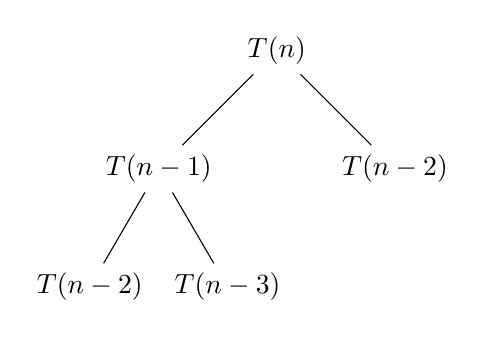
\begin{tikzpicture}[level distance=1.5cm,
    level 1/.style={sibling distance=3cm},
    level 2/.style={sibling distance=1.75cm}]
    \node {$T(n)$}
        child {node {$T(n-1)$}
            child {node {$T(n-2)$}}
            child {node {$T(n-3)$}}
        }
        child {node {$T(n-2)$}};
\end{tikzpicture}
\end{center}    
This tree will have a depth of $i$ and at every point branches by into 
two at every node.  Hence the \BigO{2^{i}} calculations. 

\subsubsection*{B:}
To show that only \BigO{n^2} operations are needed if every duplicate
$T(i)$ is calculated only once, begin by expanding the sum in the 
recurrence.
\[
T(n) = \sum_{i=1}^{n-1}T(i)T(i-1)
\]
\[ 
T(n) = T(1)T(0) + T(2)T(1) + T(3)T(2)\dots
+ T(n-2)T(n-3) + T(n-1)T(n-2)
\]
Since every $T(i)$ will only be calculated once, following sequence
can be observed by counting the number of operations needed to determine
each $T(i)$.

\begin{center}
    \begin{tabular}{c| c c c c c}
    T (i) & T (2) & T (3) & T (4) & T (5) & T (6) \\ \hline  
    Ops & 1 & 3 & 5 & 7 & 9 \\
    \end{tabular}
\end{center}
It can be shown that the $T(i+1)$ element of the sum requires two additional
operations to calculate: \textit{a multiplication and an addition}.  Hence,
this sequence will continue.  It can be proven inductively that a closed
form expression for the sum of operations required is $n^2$.  Therefore,
in this case \BigO{n^2} operations are required. 

\subsubsection*{C:}
A \BigO{n} algorithm can be derived from the original recurrence
relationship by first eliminating the summation by calculating
$T(n+1)$ in the following manner.
\[
T(n+1) = \sum_{i=1}^{n}T(i)T(i-1)
\]
\[
T(n) = \sum_{i=1}^{n-1}T(i)T(i-1)
\]
\[
T(n+1) - T(n) = \sum_{i=1}^{n}T(i)T(i-1) - \sum_{i=1}^{n-1}T(i)T(i-1)  
\]
$T(n+1)$ and $T(n)$ overlap for all values $i:1\leq i\leq n-1$, therefore
subtracting the two sums leaves only the the final in the sum for $T(n+1)$.
\[
T(n+1) - T(n) = T(n)T(n-1)
\] 
The values for n can be shifted by setting $n = m-1$.
\[
T(m) - T(m-1) = T(m-1)T(m-2)
\]
However, the label $m$ is without meaning, so label $m=n$.
\[
T(n) - T(n-1) = T(n-1)T(n-2)
\]
Equivalently,
\[
T(n) = T(n-1)[1+T(n-2)]
\]
This expression is easily expressed as a single \BigO{n} loop.\\\\
\begin{algorithm}[H]
$Array:\ T$\\
$T[0] = 2$\\
$T[1] = 2$\\
\For{$i\leftarrow 2$ to $n$}
{$T[i] = T[i-1]*(1+T[i-2])$}
$Output:\ T[n]$
\end{algorithm}
\end{document}
